%%%%%%%%%%%%%%%%%%%%%%%%%%%%%%%%%%%%%%%%%
% Beamer Presentation
% LaTeX Template
% Version 1.0 (10/11/12)
%
% This template has been downloaded from:
% http://www.LaTeXTemplates.com
%
% License:
% CC BY-NC-SA 3.0 (http://creativecommons.org/licenses/by-nc-sa/3.0/)
%
%%%%%%%%%%%%%%%%%%%%%%%%%%%%%%%%%%%%%%%%%

%----------------------------------------------------------------------------------------
%	PACKAGES AND THEMES
%----------------------------------------------------------------------------------------

\documentclass{beamer}

\mode<presentation> {

% The Beamer class comes with a number of default slide themes
% which change the colors and layouts of slides. Below this is a list
% of all the themes, uncomment each in turn to see what they look like.

%\usetheme{default}
%\usetheme{AnnArbor}
%\usetheme{Antibes}
%\usetheme{Bergen}
%\usetheme{Berkeley}
%\usetheme{Berlin}
%\usetheme{Boadilla}
%\usetheme{CambridgeUS}
%\usetheme{Copenhagen}
%\usetheme{Darmstadt}
%\usetheme{Dresden}
%\usetheme{Frankfurt}
%\usetheme{Goettingen}
%\usetheme{Hannover}
%\usetheme{Ilmenau}
%\usetheme{JuanLesPins}
%\usetheme{Luebeck}
\usetheme{Madrid}
%\usetheme{Malmoe}
%\usetheme{Marburg}
%\usetheme{Montpellier}
%\usetheme{PaloAlto}
%\usetheme{Pittsburgh}
%\usetheme{Rochester}
%\usetheme{Singapore}
%\usetheme{Szeged}
%\usetheme{Warsaw}

% As well as themes, the Beamer class has a number of color themes
% for any slide theme. Uncomment each of these in turn to see how it
% changes the colors of your current slide theme.

%\usecolortheme{albatross}
%\usecolortheme{beaver}
%\usecolortheme{beetle}
%\usecolortheme{crane}
%\usecolortheme{dolphin}
%\usecolortheme{dove}
%\usecolortheme{fly}
%\usecolortheme{lily}
%\usecolortheme{orchid}
%\usecolortheme{rose}
%\usecolortheme{seagull}
%\usecolortheme{seahorse}
%\usecolortheme{whale}
%\usecolortheme{wolverine}

%\setbeamertemplate{footline} % To remove the footer line in all slides uncomment this line
%\setbeamertemplate{footline}[page number] % To replace the footer line in all slides with a simple slide count uncomment this line

%\setbeamertemplate{navigation symbols}{} % To remove the navigation symbols from the bottom of all slides uncomment this line
}

\usepackage{graphicx} % Allows including images
\usepackage{booktabs} % Allows the use of \toprule, \midrule and \bottomrule in tables
\graphicspath{ {../res/} }%setta il path predefinito per le immagini
\usepackage[utf8]{inputenc}
\usepackage{hyperref}

%----------------------------------------------------------------------------------------
%	TITLE PAGE
%----------------------------------------------------------------------------------------

\title[Docker]{Docker - Build, Ship and Run Any App, Anywhere. } % The short title appears at the bottom of every slide, the full title is only on the title page

\author{Federico Naldini} % Your name
\institute[Unibo] % Your institution as it will appear on the bottom of every slide, may be shorthand to save space
{
Alma Mater Studiorum - Università di Bologna, Cesena. \\ % Your institution for the title page
\medskip
\textit{federico.naldini3@studio.unibo.it} % Your email address
}
\date{30/05/2018} % Date, can be changed to a custom date

\begin{document}

\begin{frame}
\titlepage % Print the title page as the first slide
\end{frame}

%------------------------------------------------
\begin{frame}
\frametitle{Overview} % Table of contents slide, comment this block out to remove it
\tableofcontents % Throughout your presentation, if you choose to use \section{} and \subsection{} commands, these will automatically be printed on this slide as an overview of your presentation
\end{frame}
%------------------------------------------------
%----------------------------------------------------------------------------------------
%	PRESENTATION SLIDES
%----------------------------------------------------------------------------------------

%------------------------------------------------
\section{La piattaforma Docker} % Sections can be created in order to organize your presentation into discrete blocks, all sections and subsections are automatically printed in the table of contents as an overview of the talk
%------------------------------------------------

\subsection{Introduzione ai \textit{containers}}

%\subsection{Architettura del sistema Docker} % A subsection can be created just before a set of slides with a common theme to further break down your presentation into chunks

%\subsection{\textit{Docker Swarm Mode}}


\begin{frame}
\frametitle{Che cos'è un \textit{container}?}
Un \textit{container} è una forma di virtualizzazione a livello di sistema operativo, in alternativa alle classiche macchine virtuali(\textit{VM}).\\
A differenza delle \textit{VM} , l'idea dietro all'approccio a \textit{containers} è di virtualizzare solo i componenti necessari, condividendo le restanti risorse con altri \textit{containers}, \textit{VM} e sistemi operativi fisici.
\end{frame}

%------------------------------------------------

\begin{frame}
\frametitle{Vantaggi dell'approccio a  \textit{containers}}
\begin{itemize}
\item Buon supporto alla scalabilità.
\item Isolamento tra i vari  \textit{containers},anche se in esecuzione sullo stesso insieme di risorse(utilizzando feature come  \textit{Namespaces}, presente nel Kernel Linux).
\item Controllo rigoroso sull'utilizzo delle risorse fisiche(sfruttando \textit{CGroups}, altra feature del Kernel Linux)
\item Overhead di virtualizzazione minimo, grazie alla riduzione del numero di layer necessari.
\end{itemize}
\end{frame}

%-----------------------------------------------
\begin{frame}
\frametitle{Layers di virtualizzazione necessari}
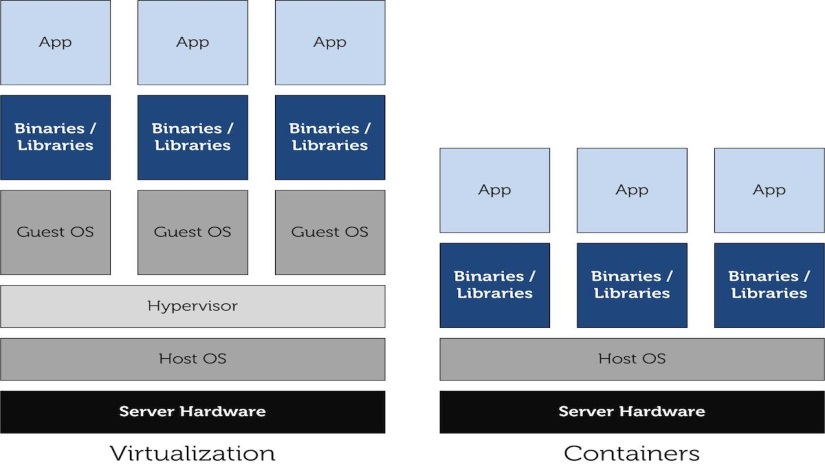
\includegraphics[width=\textwidth]{pic1}
\end{frame}

%------------------------------------------------

\subsection{Architettura del sistema Docker} % A subsection can be created just before a set of slides with a common theme to further break down your presentation into chunks

%-----------------------------------------------
\begin{frame}
\frametitle{Docker, che cos'è?}
Il progetto open source Docker viene rilasciato nel 2013 da una compagnia chiamata dotCloud, che lavorava su software di tipo PAAS (Platform as a service) per il cloud computing.\\
Docker si pone come obbiettivo di automatizzare lo sviluppo di applicazioni all’interno di containers software, sfruttando tutti i vantaggi di una virtualizzazione a livello di sistema operativo; per riuscire a fare ciò, si avvale delle funzionalità di isolamento presenti nel kernel Linux, come ad esempio cgroups, utilizzato per la gestione di risorse fisiche, e namespaces, che invece garantiscono un isolamento a livello di processo.
\end{frame}


\begin{frame}
\frametitle{ \textit{Docker Engine}}
Cuore della piattaforma è il modulo \textit{Docker Engine}, composto da tre sottomoduli:
\begin{block}{ \textit{Docker Client}}
Fornisce un insieme di comandi all’utente per poter istruire il  \textit{Docker Daemon} sul da farsi, utilizzando \texttt{API RESTful} proprietarie.
\end{block}

\begin{block}{\textit{Docker Daemon}}
Un processo demone eseguito in background su un host locale o remoto, si occupa della maggior parte del lavoro, gestendo sotto comando tutti gli oggetti del sistema.
\end{block}

\begin{block}{\textit{Docker Registry}}
Registro pubblico o privato, a cui \textit{Docker Daemon} accede per recuperare le immagini necessarie al funzionamento dei container
\end{block}
\end{frame}

%------------------------------------------------


%------------------------------------------------

\begin{frame}
\frametitle{ \textit{Docker Engine}}
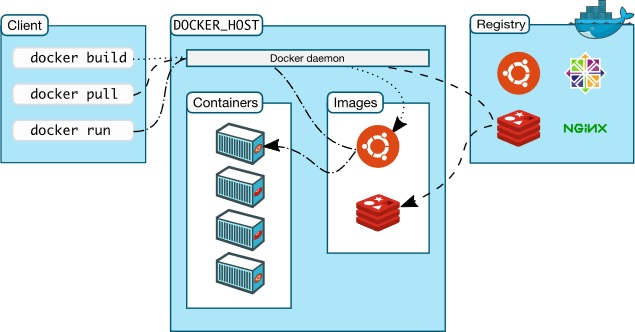
\includegraphics[width=\textwidth]{pic2}
\end{frame}

%------------------------------------------------

\subsection{Costruzione di un \textit{container} Docker}

\begin{frame}
\frametitle{Creazione di un \textit{container}}
Un  \textit{container} deve essere sempre generato da una \texttt{Docker Image}.\\
Le  \textit{best practices} di Docker associano ogni immagine a un \texttt{Dockerfile}, un file testuale che contiene le istruzioni da eseguire per generare l'immagine
\end{frame}

\begin{frame}
\frametitle{\texttt{Dockerfile}}
Ogni \texttt{Dockerfile} è strutturato in tre sezioni
\begin{block}{ \texttt{FROM}}
Specifica l'immagine da utilizzare come base.
\end{block}

\begin{block}{\texttt{RUN}}
Qui vengono indicati i comandi da eseguire sull'immagine base per ottenere il risultato desiderato.
\end{block}

\begin{block}{\texttt{CMD}}
Si piò specificare una singola istruzione, tale comando sarà eseguito all'avvio del \textit{container}
\end{block}
\end{frame}

%------------------------------------------------
\begin{frame}[fragile] % Need to use the fragile option when verbatim is used in the slide
\frametitle{Dockerfile:un esempio}
\begin{block}{\textit{Dockerfile}}
\begin{verbatim}
FROM library/openjdk:latest

EXPOSE 8080
RUN git clone
 https://gitlab.com/das-lab/lpaas/lpaas-ws.git &&\
cd lpaas-ws &&\
chmod u+x gradlew &&\
printf '#!/bin/bash\n' >> script.sh &&\
echo "cd /lpaas-ws\n ./gradlew run task" >> script.sh &&\
chmod u+x script.sh &&\
./gradlew build

CMD ["/lpaas-ws/script.sh"]
\end{verbatim}
\end{block}
\end{frame}

%------------------------------------------------
\section{Live demo}
\begin{frame}
\Huge{\centerline{Live demo}}
\end{frame}

%-------------------------------------------------
\begin{frame}[fragile]
\frametitle{Primi passi}

\begin{block}{Installazione della piattaforma(per tutti gli OS)}
\href{https://docs.docker.com/install}{https://docs.docker.com/install/}
\end{block}

\begin{block}{Verifica della corretta installazione(da eseguire su una shell)}
\begin{verbatim}
docker run hello-world
\end{verbatim}
\end{block}
\end{frame}
%-----------------------------------------------------
\begin{frame}[fragile]
\frametitle{Una semplice bash}
\begin{block}{Ubuntu bash}
\begin{verbatim}
docker run -ti ubuntu
\end{verbatim}
\end{block}
\end{frame}

%-------------------------------------------------------

\begin{frame}[fragile]
\frametitle{NodeJS}
\begin{block}{Un semplice container che manda in esecuzione un'app}
\begin{verbatim}
docker run -p 3000:3000 tirocigno/nodejssampleapp
\end{verbatim}
\end{block}
\end{frame}







\begin{frame}
\Huge{\centerline{Grazie per l'attenzione!}}
\end{frame}

%----------------------------------------------------------------------------------------

\end{document}
